For a circular orbit, we can equate the centripetal force $F_{\rm c,i}= m_ir_i\dot{\theta}^2$ to the gravitational force $F_{\rm g}=Gm_1m_2/r^2$, and solve for $\dot{\theta}^2$ in order to derive Kepler's Third Law in the form
\begin{equation}\label{eq:Chap1:keplerThirdLaw}
	\dot{\theta}^2 = \dfrac{G M}{r^3}.
\end{equation}

Equation \ref{eq:Chap1:keplerThirdLaw} is Kepler's Third Law.

\begin{figure}
	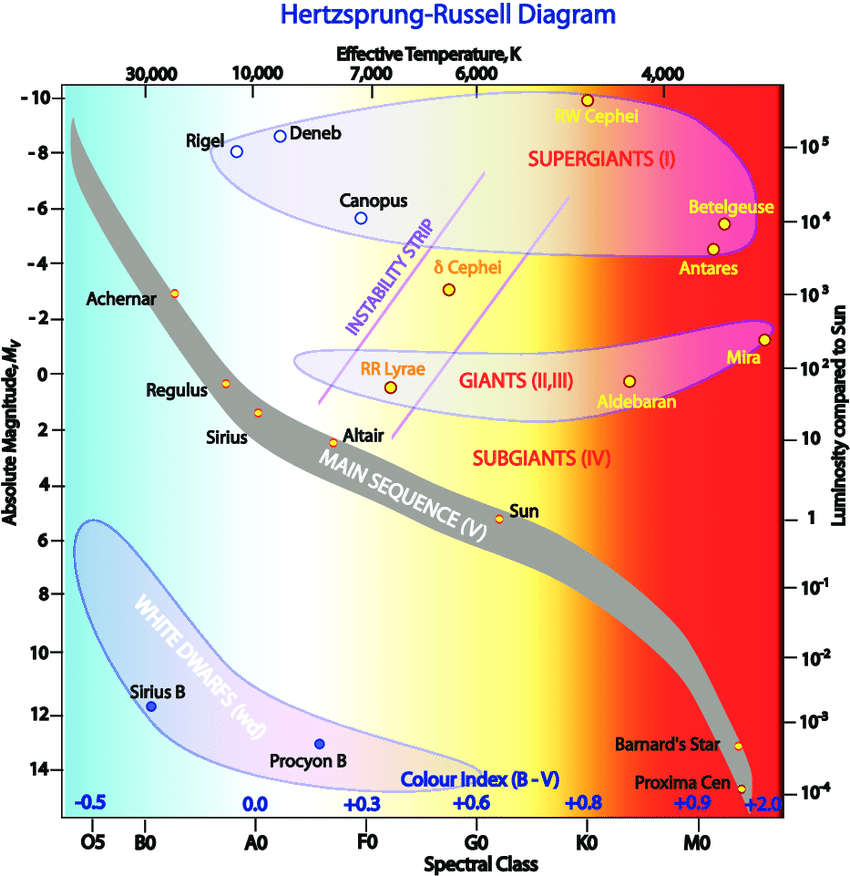
\includegraphics[width=\textwidth]{HRDAlthaus.png}
\caption[HR Diagram]{
\ac{HR} diagram as shown in figure 1 of \citet{Althaus2010}.
}
		\label{fig:Chap1:HRDAlthaus}
\end{figure}


